\lecture{25}{1. December 2025}{Mohr's circle}

\begin{problemwithimage}{f14_45}{14-45}
  The rotor shaft of the helicopter is subjected to the tensile force and torque shown when the rotor blades provide the lifting force to suspend the helicopter at midair.
  If the shaft has a diameter of \qty{150}{\mm}, determine the principal stress and maximum in-plane shear stress at a pint located on the surface of the shaft.
\end{problemwithimage}

\begin{derivation}
  The axial stress in the shaft can be found using:
  \begin{equation*}
    \sigma = \frac{P}{A} = \frac{\qty{225}{\kN}}{\pi \cdot \frac{\left( \qty{150}{\mm}  \right)^2}{4}} = \qty{12,73}{\MPa}
  .\end{equation*}
  
  The torsional shear stress at the surface is:
  \begin{equation*}
    \tau = \frac{T\rho}{J}
  .\end{equation*}
  For a solid circular shaft we have
  \begin{equation*}
    J = \frac{\pi}{2} c^{4} = \frac{\pi}{2} \frac{d^{4 }}{16}
  .\end{equation*}
  Which means:
  \begin{equation*}
    \tau = \frac{T \cdot \frac{d}{2}}{J} = \frac{16 T}{\pi d^3} = \frac{16 \cdot \qty{15}{\kN.\m} }{\pi \cdot \left( \qty{150}{\mm}  \right)^3} = \qty{22,64}{\MPa} 
  .\end{equation*}
  
  So at a surface point, the plane-stress state is:
  \begin{equation*}
    \sigma_x = \qty{12,73}{\MPa}, \qquad \sigma_y = \qty{0}{\MPa}, \qquad \tau_{xy} = \qty{22,64}{\MPa}
  .\end{equation*}

  To draw the Mohr's circles we use:
  \begin{align*}
    \sigma_{\mathrm{avg}} &= \frac{\sigma_x + \sigma_y}{2} = \frac{\qty{12,73}{\MPa}}{2} = \qty{6,365}{\MPa} \\
    R &= \sqrt{\left( \frac{\sigma_x - \sigma_y}{2} \right)^2 + \tau_{xy}^2} \\
    &= \sqrt{\left( \qty{6.365}{\MPa}  \right)^2 + \left( \qty{22.64}{\MPa}  \right)^2} \\
    &= \qty{23,5}{\MPa} 
  .\end{align*}
  So,
  \begin{equation*}
    \sigma_{1,2} = \sigma_{\mathrm{avg}} \pm R = \qty{6,365}{\MPa} ´\pm \qty{23,5}{\MPa} \implies \sigma_1 = \qty{29,865}{\MPa}, \sigma_2 = \qty{-17,135}{\MPa} 
  .\end{equation*}
  The maximum in-plane shear is just the Mohr radius:
  \begin{equation*}
    \tau_{\mathrm{max}, \mathrm{in-plane}} = R = \qty{23,5}{\MPa} 
  .\end{equation*}
\end{derivation}

\finalresult{
\begin{aligned}
  \sigma_1 &= \qty{29,865}{\MPa} \\
  \sigma_2 &= - \qty{17,135}{\MPa} \\
  \tau_{\mathrm{max}, \mathrm{in-plane}} &= \qty{23,5}{\MPa} 
.\end{aligned}
}

\begin{problemwithimage}{f14_49}{14-49}
  Draw the three Mohr's circles that describe the following state of stress.
\end{problemwithimage}

\begin{derivation}
  We take the right-hand direction to be $+x$ meaning $\sigma_x = \qty{400}{\MPa}$ and the downwards axis to be $-y$ meaning $\sigma_y = - \qty{300}{\MPa}$.
  Nothing is shown in the $z$ direction, so $\sigma_z = \qty{0}{\MPa}$, $\tau_{xy} = \tau_{yz} = \tau_{zx} = \qty{0}{\MPa}$. 

  We therefore get the three circles $12$, $23$, and $31$.

  For circle $12$ which is between $\sigma_x = \qty{400}{\MPa}$ and $\sigma_z = \qty{0}{\MPa}$ we get:
  \begin{align*}
    C_{12} &= \frac{\sigma_x + \sigma_z}{2} = \frac{\qty{400}{\MPa}}{2} = \qty{200}{\MPa} \\
    R_{12} &= \frac{\sigma_x - \sigma_z}{2} = \frac{\qty{400}{\MPa}}{2} = \qty{200}{\MPa}
  .\end{align*}
  
  For circle $23$ which is between $\sigma_z = \qty{0}{\MPa}$ and $\sigma_y = - \qty{300}{\MPa}$ we get:
  \begin{align*}
    C_{23} &= \frac{\sigma_z + \sigma_y}{2} = \frac{\qty{-300}{\MPa} }{2} =  \qty{-150}{\MPa} \\
    R_{23} &= \frac{\sigma_z - \sigma_y}{2} = \frac{\qty{300}{\MPa} }{2} = \qty{150}{\MPa} 
  .\end{align*}

  And for circle $31$ between $\sigma_y = - \qty{300}{\MPa}$ and $\sigma_x = \qty{400}{\MPa} $ we get
  \begin{align*}
    C_{31} &= \frac{\sigma_x + \sigma_y}{2} = \frac{\qty{400}{\MPa} - \qty{300}{\MPa} }{2} = \qty{50}{\MPa}  \\
    R_{31} &= \frac{\sigma_x - \sigma_y}{2} = \frac{\qty{400}{\MPa} + \qty{300}{\MPa} }{2} = \qty{350}{\MPa} 
  .\end{align*}

  On \Cref{fig:f14_49mohr} the Mohr's circles are sketches.

  \begin{figure} [ht]
    \centering
    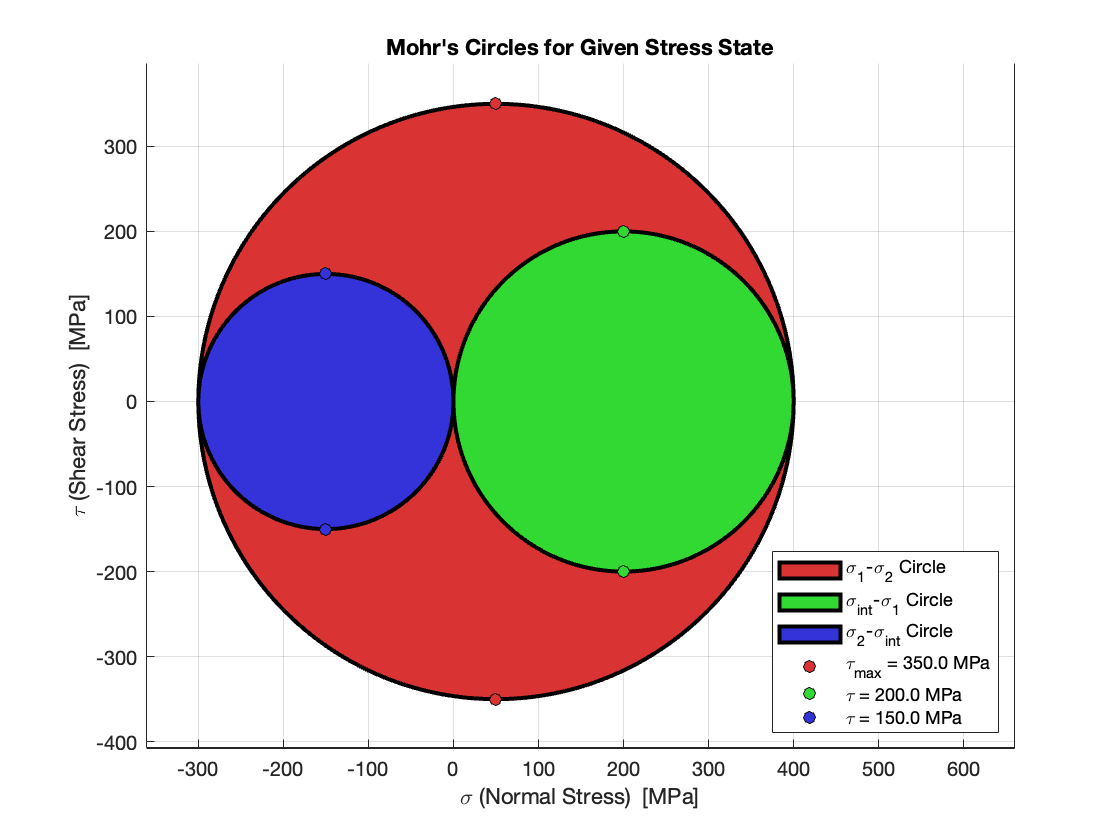
\includegraphics[width=\linewidth]{./figures/f14_49mohr.png}
    \caption{Mohr's circles for the given state.}
    \label{fig:f14_49mohr}
  \end{figure}
\end{derivation}

\clearpage

\begin{problemwithimage}{f14_51}{14-51}
  The stress at a point is shown on the element.
  Determine the principal stress and absolute maximal shear stress.
\end{problemwithimage}

\begin{derivation}
  The stress state this time is:
  \begin{align*}
    \sigma_x &= \qty{0}{\MPa}, & \sigma_y &= \qty{30}{\MPa}, & \sigma_z &= \qty{120}{\MPa} \\
    \tau_{xy} &= \qty{0}{\MPa}, & \tau_{xz} &= \qty{0}{\MPa}, &\tau_{yz} &= \qty{70}{\MPa} 
  .\end{align*}
  
  This means that our Mohr's circles have centers at:
  \begin{align*}
    C_{12} &= \frac{\sigma_{x} + \sigma_z}{2} = \frac{\qty{120}{\MPa}}{2} = \qty{60}{\MPa}  \\
    C_{23} &= \frac{\sigma_z + \sigma_y}{2} = \frac{\qty{120}{\MPa} + \qty{30}{\MPa}}{2} = \qty{75}{\MPa}  \\
    C_{31} &= \frac{\sigma_x + \sigma_y}{2} = \frac{\qty{30}{\MPa}}{2} = \qty{15}{\MPa}
  .\end{align*}
  and radiusses of:
  \begin{align*}
    R_{12} &= \sqrt{\left( \frac{\sigma_x - \sigma_y}{2} \right)^2 + \tau_{xy}^2} = \sqrt{\left( \qty{15}{\MPa}  \right)^2} = \qty{15}{\MPa} \\
    R_{23} &= \sqrt{\left( \frac{\sigma_y - \sigma_z}{2}\right)^2 + \tau_{yz}^2} = \sqrt{\left( \qty{45}{\MPa}  \right)^2 + \left( \qty{70}{\MPa} \right)^2} = \qty{83,21}{\MPa} \\
    R_{31} &= \sqrt{\left(\frac{\sigma_x - \sigma_z}{2}\right)^2 + \tau_{xz}^2} = \qty{60}{\MPa}
  .\end{align*}
  And the three produced circles are depicted on \cref{fig:f14_51mohr}.

  \begin{figure} [ht]
    \centering
    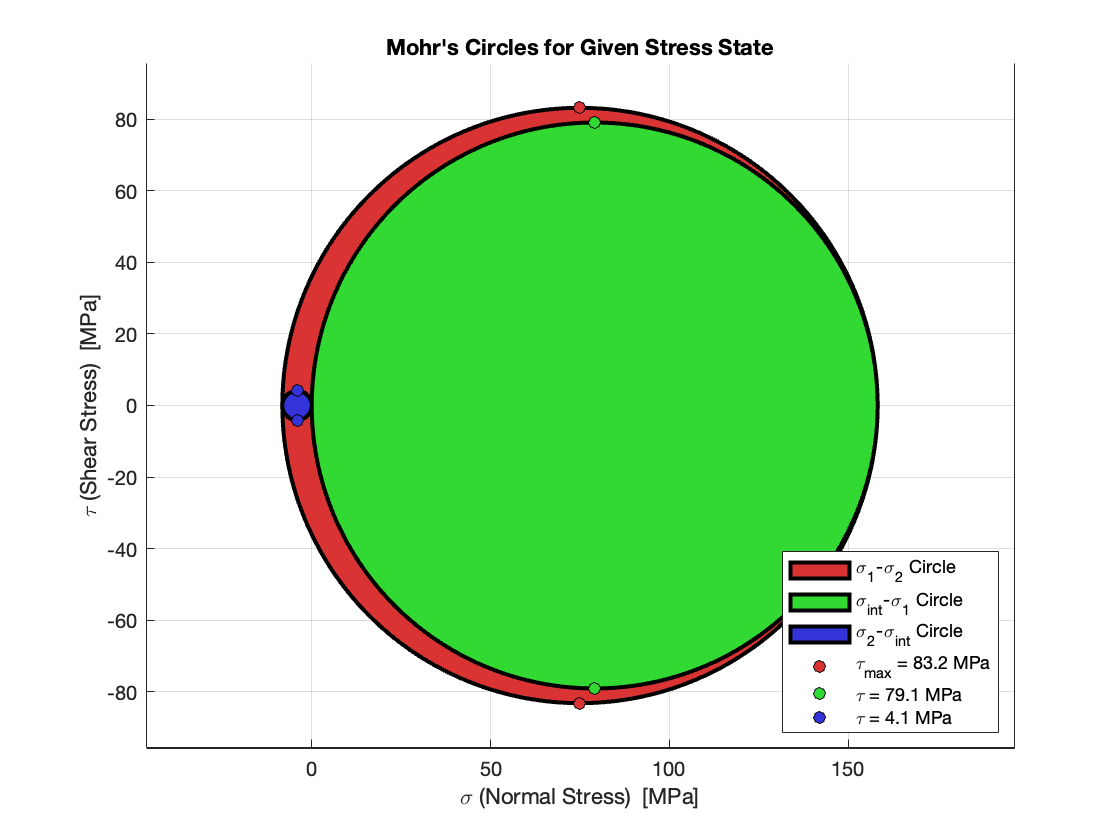
\includegraphics[width=\linewidth]{./figures/f14_51mohr.png}
    \caption{Mohr's circles for the given stress state.}
    \label{fig:f14_51mohr}
  \end{figure}

  The principal stresses are found using the circle with the biggest Mohr radius::
  \begin{equation*}
    \sigma_{1,3} = \sigma_C \pm R = \qty{75}{\MPa} \pm \qty{83,21}{\MPa} \implies \sigma_1 = \qty{158,21}{\MPa}, \sigma_3 = - \qty{8,21}{\MPa}
  .\end{equation*}
  Furthermore $\sigma_2 = 0$.

  Lastly, the maximum in-plane shear corresponds to the biggest Mohr radius:
  \begin{equation*}
    \tau_{\mathrm{max}, \mathrm{in-plane}} = R_{23} = \qty{83,21}{\MPa} 
  .\end{equation*}
\end{derivation}

\finalresult{
\begin{aligned}
  \sigma_1 &= \qty{158,21}{\MPa}  \\
  \sigma_2 &= \qty{0}{\MPa}  \\
  \sigma_{3} &= \qty{-8,21}{\MPa} \\
  \tau_{\mathrm{max}, \mathrm{in-plane}} &= \qty{83,21}{\MPa}
.\end{aligned}
}
